\documentclass[a4paper, 12pt]{article}
\usepackage{eurosym}
\usepackage{pdflscape}
\usepackage{pgfgantt}
\usepackage{pgfplots}
\usepackage{booktabs}
\usepackage{longtable}


\newcommand{\templates}{../../template}
\usepackage[a4paper, margin=2.5cm]{geometry}

\usepackage{enumitem}
\setlist[itemize]{noitemsep}
\setlist[enumerate]{noitemsep}

\let\oldpar\paragraph
\renewcommand{\paragraph}[1]{\oldpar{#1\\}\noindent}

% Avoid dots in the table of contents, it mess with the gulpease calculation
\makeatletter
\renewcommand{\@dotsep}{10000} 
\makeatother
\usepackage{graphicx}
\usepackage{hyperref}
\usepackage{makecell}
\usepackage{fancyhdr}

\newcommand{\settitolo}[1]{\newcommand{\titolo}{#1\\}}
\newcommand{\setprogetto}[1]{\newcommand{\progetto}{#1\\}}
\newcommand{\setcommittenti}[1]{\newcommand{\committenti}{#1\\}}
\newcommand{\setredattori}[1]{\newcommand{\redattori}{#1\\}}
\newcommand{\setrevisori}[1]{\newcommand{\revisori}{#1\\}}
\newcommand{\setresponsabili}[1]{\newcommand{\responsabili}{#1\\}}
\newcommand{\setversione}[1]{
	\ifdefined\versione\renewcommand{\versione}{#1\\}
	\else\newcommand{\versione}{#1\\}\fi
}
\newcommand{\setdestuso}[1]{\newcommand{\uso}{#1\\}}
\newcommand{\setdescrizione}[1]{\newcommand{\descrizione}{#1\\}}

\newcommand{\makefrontpage}{
	\begin{titlepage}
		\begin{center}

		
\includegraphics[width=0.4\textwidth]{\templates/4ourSquared_logo}\\

		{\Large 4OURSQUARED}\\[6pt]
		\href{mailto://4oursquared.unipd@gmail.com}{4oursquared.unipd@gmail.com}\\
		
		\ifdefined\progetto
		\vspace{1cm}
		{\Large\progetto}
		{\large\committenti}
		\else\fi
		
		\vspace{1.5cm}
		{\LARGE\titolo}
		
		\vfill
		
		\begin{tabular}{r | l}
		\multicolumn{2}{c}{\textit{Informazioni}}\\
		\hline
		
		\ifdefined\redattori
			\textit{Redattori} &
			\makecell[l]{\redattori}\\
		\else\fi
		\ifdefined\revisori
			\textit{Revisori} &
			\makecell[l]{\revisori}\\
		\else\fi
		\ifdefined\responsabili
			\textit{Responsabili} &
			\makecell[l]{\responsabili}\\
		\else\fi
		
		\ifdefined\versione
			\textit{Versione} & \versione
		\else\fi
		
		\textit{Uso} & \uso
		
		\end{tabular}
		
		\vspace{2cm}
		
		\ifdefined\descrizione
		Descrizione
		\vspace{6pt}
		\hrule
		\descrizione
		\else\fi
		\end{center}
	\end{titlepage}
}
\usepackage{hyperref}
\usepackage{array}
\usepackage{tabularx}
\usepackage{adjustbox}

\newcounter{verscount}
\setcounter{verscount}{0}
\newcommand{\addversione}[5]{
	\ifdefined\setversione
		\setversione{#1}
	\else\fi
	\stepcounter{verscount}
	\expandafter\newcommand%
		\csname ver\theverscount \endcsname{#1&#2&#3&#4&#5}
}

\newcommand{\listversioni}{
	\ifnum\value{verscount}>1
		\csname ver\theverscount \endcsname
		\addtocounter{verscount}{-1}
		\\\hline
		\listversioni
	\else
		\csname ver\theverscount \endcsname\\\hline
	\fi
}

\newcommand{\makeversioni}{
	\begin{center}
		\begin{tabularx}{\textwidth}{|c|c|c|c|X|}
		\hline
		\textbf{Versione} & \textbf{Data} & \textbf{Redattore} & \textbf{Verificatore} & \textbf{Descrizione} \\
		\hline
		\listversioni
		\end{tabularx}
	\end{center}
	\clearpage
}
\graphicspath{ {./immagini/} }

\settitolo{Analisi dei requisiti}
\setredattori{Nicolas Alberti \\ Romina Brotto \\ Erica Cavaliere \\ Francesco Ceccato }
\setdestuso{esterno}
\setdescrizione{
Questo documento si occupa di riportare un'analisi di tutti gli elementi richiesti e i vincoli da rispettare per una completa comprensione del progetto.
}


\addversione{0.0.1}{05/05/2023}{Erica Cavaliere}{Lorenzo Salami}{Stesura iniziale}
\addversione{0.0.2}{05/05/2023}{Francesco Ceccato}{Lorenzo Salami}{Inserimento di alcuni casi d'uso}
\addversione{0.0.3}{09/05/2023}{Brotto Romina}{Soldà Matteo}{Aggiunta sezioni 2, 2.1, 4, 4.1 ed inizio stesura requisiti funzionali}
\addversione{0.0.4}{10/05/2023}{Alberti Nicolas}{Brotto Romina}{Aggiunta Tabella Requisiti funzionali}
\addversione{0.0.5}{25/05/2023}{Brotto Romina}{Cavaliere Erica}{Sistemazione casi d'uso, aggiunta sottocasi e requisiti funzionali}
\addversione{0.0.6}{01/06/2023}{Brotto Romina}{Soldà Matteo}{Aggiunti sottocasi da 11.1.1 al 11.1.5 con relativi requisiti funzionali e correzione immagini use case}
\addversione{0.0.7}{04/07/2023}{Brotto Romina}{Cavaliere Erica}{Aggiunti casi d'uso mancanti, effettuate correzioni consigliate dal Committente e sistemate immagini}
\addversione{0.1.0}{20/07/2023}{Brotto Romina}{Soldà Matteo}{Verifica per RTB}
\addversione{1.0.0}{20/07/2023}{Soldà Matteo}{Brotto Romina}{Approvazione per candidatura RTB}
\addversione{1.0.1}{09/08/2023}{Brotto Romina}{Cavaliere Erica}{Aggiornamento con requisiti di Qualità e requisiti di Vincolo}


\def\pgfcalendarmonthitname#1{%
\ifcase#1 \or Gennaio\or Febbraio\or Marzo\or Aprile\or Maggio\or Giugno\or Luglio\or Agosto\or Settembre\or Ottobre\or Novembre\or Dicembre\fi%
}
\usepgfplotslibrary{dateplot}

\begin{document}
\makeindexdetails
\makefrontpage \makeversioni
\tableofcontents
\newpage
\clearpage
\makecontentsdetails{Analisi dei requisiti} 

\section{Introduzione}
\subsection{Scopo del Documento}
In questo progetto viene richiesto di creare un sistema che permetta di gestire i lampioni, accendendo una o più luci se sono presenti nelle vicinanze una o più persone o spegnendole altrimenti.\newline
Bisognerà che ci sia anche un modo per registrare i guasti degli impianti e segnalarli tramite apposita applicazione.

\subsection{Riferimenti}
\subsubsection*{Riferimenti normativi}
\begin{itemize}
    \item Capitolato d'appalto: C2; 
    \item Norme di Progetto.
\end{itemize}

\subsubsection*{Riferimenti informativi}
\begin{itemize}
    \item Slide analisi dei requisiti - Materiale didattico del corso IS;
    \item Slide diagrammi dei casi d'uso - Materiale didattico del corso IS.
\end{itemize}
\newpage
\section{Descrizione del Prodotto}
L'azienda \textit{Imola Informatica} propone attraverso il capitolato C2:
\textit{Lumos Minima}. L'obiettivo è sviluppare un sistema per l'ottimizzazione
dell'illuminazione pubblica che permetta ai gestori di sfruttare la possibilità
di regolare l'intensità di luce emessa dagli \textit{impianti luminosi\textsubscript{G}}, grazie all'utilizzo di
sensori specifici che permettono di ottenere informazioni legate all'ambiente circostante.
\subsection{Scopo del Prodotto}
Il sistema sopra citato consentirebbe di garantire sicurezza stradale e sociale, e al tempo stesso permetterebbe di risparmiare energia e quindi risorse economiche ed ambientali. Il processo è caratterizzato da operazioni effettuate dal sistema e/o dai gestori:
\begin{itemize}
    \item Rilevamento della presenza di persone in prossimità della fonte luminosa;
    \item Aumento e riduzione dell'intensità luminosa;
    \item Rilevamento automatico del guasto di un impianto di illuminazione;
    \item Segnalazione manuale del guasto di un impianto di illuminazione;
    \item Aumento e riduzione manuale dell'intensità luminosa;
    \item Inserimento e gestione di un impianto luminoso;
    \item Aumento o riduzione globale dell'intensità luminosa. 
\end{itemize}

\subsection{Parti del Prodotto}
Il prodotto si compone delle seguenti parti: % BOZZA
\begin{itemize}
    \item \textit{Landing page\textsubscript{G}} per permettere l'autenticazione dell'operatore;
    \item \textit{Web App\textsubscript{G}} con \textit{dashboard\textsubscript{G}} per visualizzare, selezionare tutti i gruppi di
    impianti luminosi ed interagire con essi;
    \item \textit{BackEnd\textsubscript{G}} server che opera effettivamente sui lampioni.
\end{itemize}
% BOZZA - DA DEFINIRE
Per ogni impianto luminoso deve essere prevista una modalità a funzionamento
automatico ed una modalità a funzionamento manuale, in cui l'operatore potrà
configurare a proprio piacimento gli elementi dell'impianto. 
\subsection{Caratteristiche utenti}
La Web App prevede due tipologie di utenti:
\begin{itemize}
    \item operatore non autenticato, che può: \begin{itemize}
        \item visualizzare la landing page;
        \item accedere al servizio previo possesso di credenziali autenticate.
    \end{itemize}
    \item operatore autenticato, che può: \begin{itemize}
        \item visualizzare tutti gli impianti luminosi gestiti dall'organizzazione;
        \item interagire con ogni impianto e modificarne il funzionamento;
        \item visualizzare eventuali errori e/o guasti.
    \end{itemize}
\end{itemize}
% BOZZA - DA DEFINIRE
Il prodotto si rivolge a tutte le organizzazioni che necessitano di gestire un
numero consistente di impianti luminosi, a loro volta composti da più elementi
quali luci e sensori. L'utente finale deve conoscere il funzionamento di tali
componenti, al fine di poter gestire nella maniera più adeguata gli impianti ed
inoltre deve saper interpretare gli errori forniti dal prodotto, per poter
correggere il funzionamento dell'impianto.

\subsection{Vincoli e preferenze}
Il proponente non impone particolari vincoli nella scelta delle tecnologie e dei linguaggi, sono stati però forniti alcui suggerimenti da prendere in considerazione:
\begin{itemize}
    \item utilizzo di React per lo sviluppo delle parti di \textit{Front-end\textsubscript{G}};
    \item utilizzo di Node JS per lo sviluppo delle parti di \textit{Back-end\textsubscript{G}};
\end{itemize}

Per il completamento del progetto il proponente richiede che siano ottenuti i
seguenti risultati:
\begin{itemize}
    \item applicazione Web Responsive che soddisfi i requisiti obblgatori
    illustrati dai casi d'uso;
    \item test che dimostrino il corretto funzionamento dei servizi e delle
    funzionalità previste, con una copertura minima dell'80\%;
    \item documentazione sulle scelte implementative e progettuali con le
    motivazioni e i problemi aperti ed eventuali soluzioni da esplorare.
\end{itemize}
Sono di interesse altri due risultati desiderabili ma non vincolanti al fine del
completamento del progetto:
\begin{itemize}
    \item cifratura di tutte le comunicazoni fra App e Server per garantire la
    validità delle informazioni;
    \item analisi riguardante sia il carico massimo supportato in numero di
    dispositivi che del servizio cloud più adatto per supportarlo
    analizzando prezzo, stabilità, del servizio ed assistenza.
\end{itemize} 
\newpage
\section{Casi d'uso}

\subsection{Diagramma dei casi d'uso}

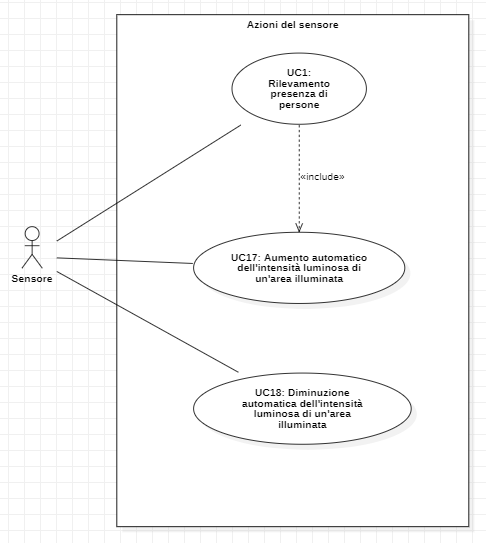
\includegraphics[scale=0.8]{diagramma_use_case_1.png}

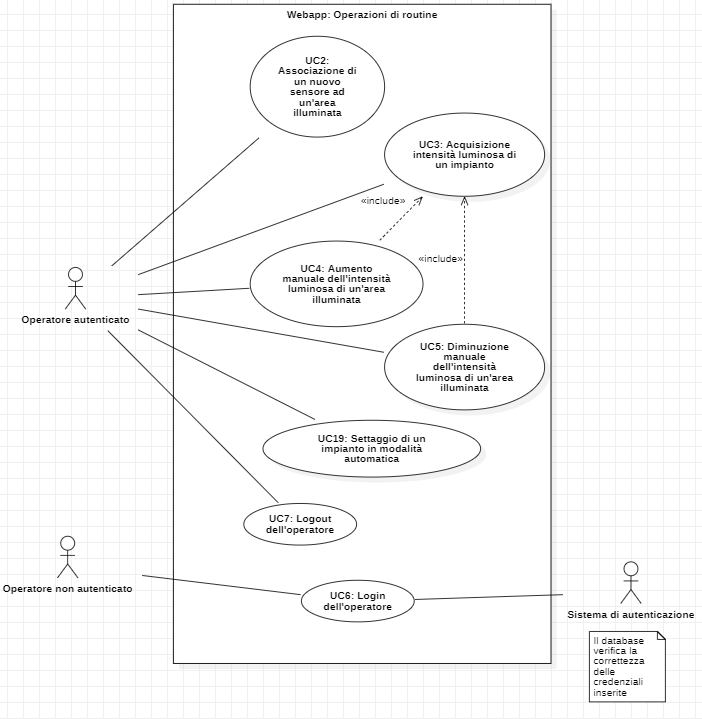
\includegraphics[scale=0.8]{diagramma_use_case_2.png}

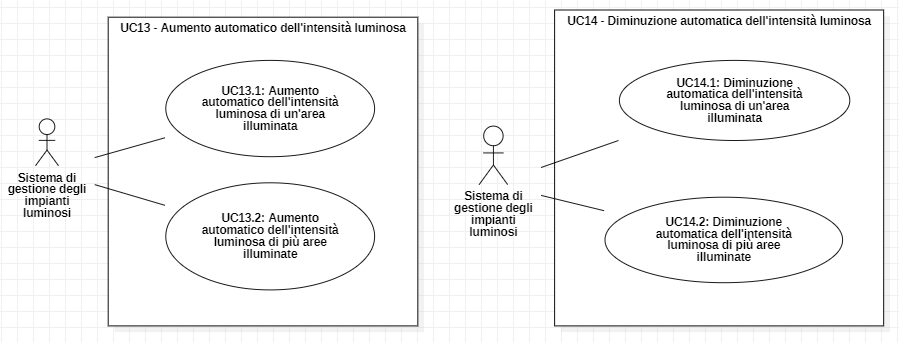
\includegraphics[scale=0.65]{diagramma_use_case_3e4.png}

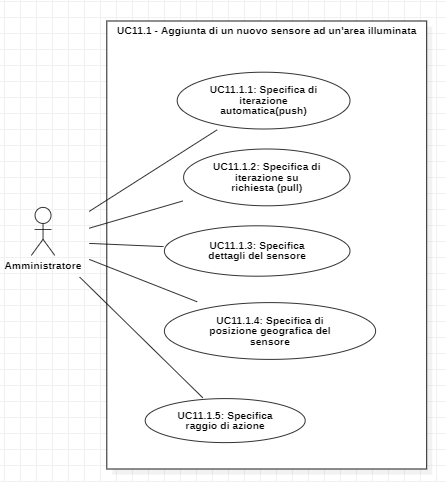
\includegraphics[scale=0.7]{diagramma_use_case_5.png}

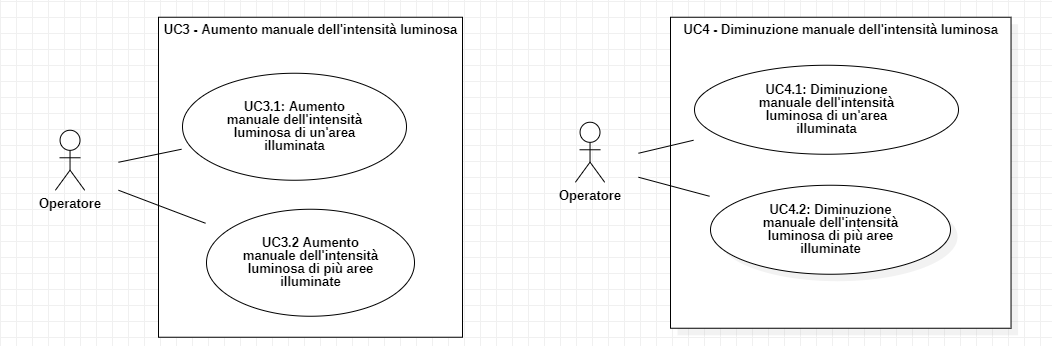
\includegraphics[scale=0.60]{diagramma_use_case_6e7.png}

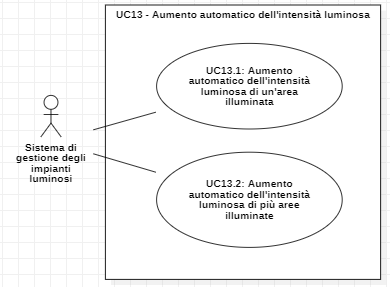
\includegraphics[scale=0.7]{diagramma_use_case_8.png}

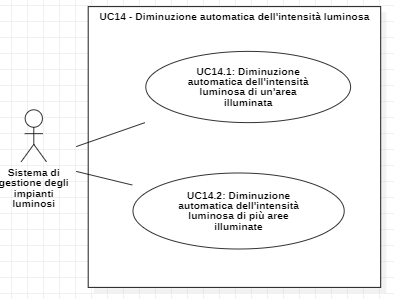
\includegraphics[scale=0.7]{diagramma_use_case_9.png}

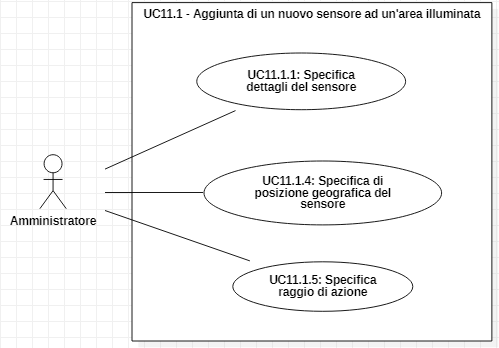
\includegraphics[scale=0.60]{diagramma_use_case_10.png}

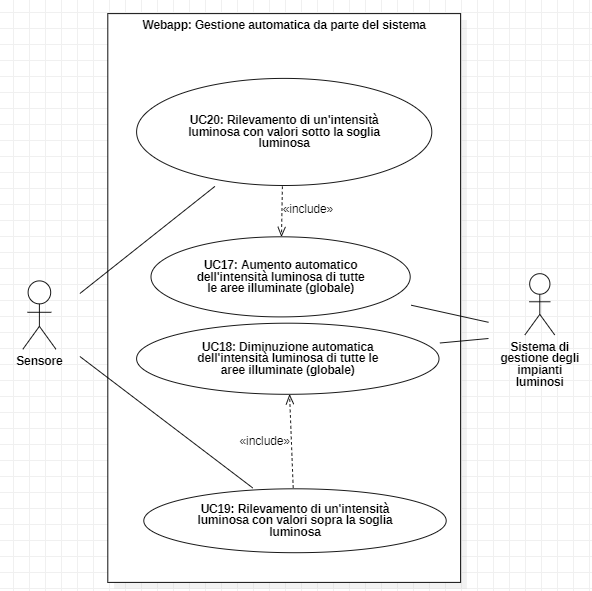
\includegraphics[scale=0.63]{diagramma_use_case_11.png}

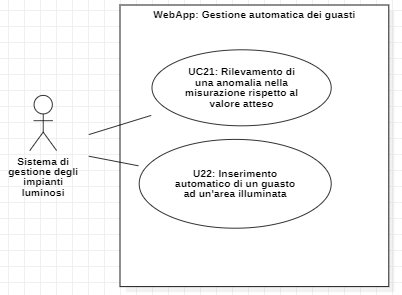
\includegraphics[scale=0.65]{diagramma_use_case_12.png}

\subsection{Attori}
\begin{itemize}
    \item Utente non autenticato: utente che non ha inserito le proprie credenziali;
    \item Utente autenticato: utente che ha inserito correttamente le credenziali;
    \item Sistema di autenticazione: sistema di controllo che permette di verificare il corretto inserimento dei dati per accedere al programma;
    \item Manutentore: legge l'elenco delle aree illumninate guaste e si occupa di segnalarle come riparate;
    \item Operatore: si occupa di gestire le aree luminose (accensioni e spegnimenti e regolazioni) e segnala i guasti presenti;
    \item Amministratore: operatore registrato che oltre a poter configurare nuove aree, può aggiungere o eliminare sensori o impianti luminosi;
    \item Sensore: dispositivo che si occupa di rilevare le persone e modificare l'intensità luminosa degli impianti di illuminazione;
    \item Sistema di gestione degli impianti luminosi: si occupa della gestione automatica dell'intensità luminosa delle aree illuminate.
\end{itemize}

\subsection{Lista dei casi d'uso}

\subsubsection{UC1 - Rilevamento presenza di persone automatico}
\textbf{Attore:} Sensore.\newline
\textbf{Attore secondario:} Sistema di Gestione degli impianti luminosi.\newline
\textbf{PRE:} l'individuo non è ancora posizionato in prossimità dell'area con lampioni, i lampioni sono spenti o con intensità luminosa settata al minimo.\newline
\textbf{POST:} l'individuo è posizionato all'interno dell'area, i lampioni illuminano l'area.\newline
\textbf{Scenario principale:}
\begin{enumerate}
    \item Il sensore rileva la presenza di uno o più individui nel raggio d'azione;
    \item Il sistema riceve in modalità \textit{push/pull\textsubscript{G}} le informazioni dal sensore;
    \item Il sistema elabora l'informazione ricevuta, aumenta l'intensità luminosa dell'area (include[UC17]) per un certo tempo;
    \item A seguire, l'intensità luminosa dell'area viene riportata al valore di default.
\end{enumerate}
\textbf{Requisiti collegati:} RF1-O\newline 

\subsubsection{UC1.1 - Rilevamento presenza di persone automatico}
\textbf{Attore:} Sensore.\newline
\textbf{PRE:} l'individuo non è ancora posizionato in prossimità dell'area con lampioni, i lampioni sono spenti.\newline
\textbf{POST:} l'individuo è posizionato all'interno dell'area, i lampioni illuminano l'area.\newline
\textbf{Scenario principale:}
\begin{enumerate}
    \item Il sensore rileva la presenza di uno o più individui nel raggio d'azione;
    \item Il sistema riceve in modalità push le informazioni dal sensore;
    \item Il sistema elabora l'informazione ricevuta, aumenta l'intensità luminosa dell'area (include[UC17]) per un certo tempo;
    \item A seguire, l'intensità luminosa dell'area viene riportata al valore di default.
\end{enumerate}
\textbf{Requisiti collegati:} RF21-O\newline

\subsubsection{UC1.2 - Rilevamento presenza di persone su richiesta}
\textbf{Attore:} Sensore.\newline
\textbf{PRE:} l'individuo non è ancora posizionato in prossimità dell'area con lampioni, i lampioni sono spenti.\newline
\textbf{POST:} l'individuo è posizionato all'interno dell'area, i lampioni illuminano l'area.\newline
\textbf{Scenario principale:}
\begin{enumerate}
    \item Il sensore rileva la presenza di uno o più individui nel raggio d'azione;
    \item Il sistema riceve in modalità pull le informazioni dal sensore;
    \item Il sistema elabora l'informazione ricevuta, aumenta l'intensità luminosa dell'area (include[UC17]) per un certo tempo;
    \item A seguire, l'intensità luminosa dell'area viene riportata al valore di default.
\end{enumerate}
\textbf{Requisiti collegati:} RF22-F\newline

\subsubsection{UC2 - Visualizzazione intensità luminosa di un'area illuminata}
\textbf{Attore:} Operatore.\newline
\textbf{PRE:} un'\textit{area illuminata\textsubscript{G}} configurata illumina con un intensità iniziale arbitraria.\newline
\textbf{POST:} l'area illuminata summenzionata illumina con una precisa intensità finale.\newline
\textbf{Scenario principale:}
\begin{enumerate}
    \item L'operatore accede al sistema;
    \item L'operatore effettua il login con proprie credenziali;
    \item Il sistema acquisisce l'elenco di tutte le aree illuminate;
    \item L'operatore seleziona una aree illuminate;
    \item L'operatore imposta un valore di intensità luminosa per gli impianti nell'area selezionata;
    \item Il sistema configura tutti gli impianti selezionati all'intensità desiderata.
\end{enumerate}
\textbf{Requisiti collegati:} RF2-O\newline



\subsubsection{UC3 - Aumento manuale dell'intensità luminosa}
\textbf{Attore:} Operatore.\newline
\textbf{PRE:} un'area illuminata configurata illumina con un intensità iniziale arbitraria.\newline
\textbf{POST:} l'area illuminata summenzionata illumina con una precisa intensità finale.\newline
\textbf{Scenario principale:}
\begin{enumerate}
    \item L'operatore accede al sistema;
    \item L'operatore effettua il login con proprie credenziali;
    \item Il sistema mostra l'elenco di tutte le aree illuminate;
    \item L'operatore seleziona un'area illuminata;
    \item L'operatore imposta un valore maggiore di intensità luminosa per tutti gli impianti nell'area selezionata;
    \item Il sistema configura tutti gli impianti selezionati all'intensità desiderata.
\end{enumerate}
\textbf{Requisiti collegati:} RF3-O\newline

\subsubsection{UC3.1 - Aumento manuale dell'intensità luminosa di un'area illuminata}
\textbf{Attore:} Operatore.\newline
\textbf{PRE:} un'area illuminata configurata illumina con un intensità iniziale arbitraria.\newline
\textbf{POST:} l'area illuminata summenzionata illumina con una precisa intensità finale.\newline
\textbf{Scenario principale:}
\begin{enumerate}
    \item L'operatore accede al sistema;
    \item L'operatore effettua il login con proprie credenziali;
    \item Il sistema mostra l'elenco di tutte le aree illuminate;
    \item L'operatore seleziona un'area illuminata;
    \item L'operatore imposta un valore maggiore di intensità luminosa per tutti gli impianti nell'area selezionata;
    \item Il sistema configura tutti gli impianti selezionati all'intensità desiderata.
\end{enumerate}
\textbf{Requisiti collegati:} RF23-O\newline

\subsubsection{UC3.2 - Aumento manuale dell'intensità luminosa di più aree illuminate}
\textbf{Attore:} Operatore.\newline
\textbf{PRE:} le aree luminose configurate illuminano con un intensità iniziale arbitraria.\newline
\textbf{POST:} le aree luminose summenzionate illuminano con una precisa intensità finale.\newline
\textbf{Scenario principale:}
\begin{enumerate}
    \item L'operatore accede al sistema;
    \item L'operatore effettua il login con proprie credenziali;
    \item Il sistema mostra l'elenco di tutte le aree illuminate;
    \item L'operatore seleziona più aree illuminate;
    \item L'operatore imposta un valore maggiore di intensità luminosa per tutti gli impianti nelle aree selezionate;
    \item Il sistema configura tutti gli impianti selezionati all'intensità desiderata.
\end{enumerate}
\textbf{Requisiti collegati:} RF24-F\newline

\subsubsection{UC4 - Diminuzione manuale dell'intensità luminosa}
\textbf{Attore:} Operatore.\newline
\textbf{PRE:} un'area illuminata configurata illumina con un intensità iniziale arbitraria.\newline
\textbf{POST:} l'area illuminata summenzionata illumina con una precisa intensità finale.\newline
\textbf{Scenario principale:}
\begin{enumerate}
    \item L'operatore accede al sistema;
    \item L'operatore effettua il login con proprie credenziali;
    \item Il sistema mostra elenco di tutte le aree illuminate;
    \item L'operatore seleziona un'area illuminata;
    \item L'operatore imposta un valore minore di intensità luminosa per tutti gli impianti nell'area selezionata;
    \item Il sistema configura tutti gli impianti selezionati all'intensità desiderata.
\end{enumerate}
\textbf{Requisiti collegati:} RF4-O\newline

\subsubsection{UC4.1 - Diminuzione manuale dell'intensità luminosa di un'area illuminata}
\textbf{Attore:} Operatore.\newline
\textbf{PRE:} un'area illuminata configurata illumina con un intensità iniziale arbitraria.\newline
\textbf{POST:} l'area illuminata summenzionata illumina con una precisa intensità finale.\newline
\textbf{Scenario principale:}
\begin{enumerate}
    \item L'operatore accede al sistema;
    \item L'operatore effettua il login con proprie credenziali;
    \item Il sistema mostra elenco di tutte le aree illuminate;
    \item L'operatore seleziona un'area illuminata;
    \item L'operatore imposta un valore minore di intensità luminosa per tutti gli impianti nell'area selezionata;
    \item Il sistema configura tutti gli impianti selezionati all'intensità desiderata.
\end{enumerate}
\textbf{Requisiti collegati:} RF25-O\newline

\subsubsection{UC4.2 - Diminuzione manuale dell'intensità luminosa di più aree illuminate}
\textbf{Attore:} Operatore.\newline
\textbf{PRE:} le aree luminose configurate illuminano con un intensità iniziale arbitraria.\newline
\textbf{POST:} le aree luminose summenzionate illuminano con una precisa intensità finale.\newline
\textbf{Scenario principale:}
\begin{enumerate}
    \item L'operatore accede al sistema;
    \item L'operatore effettua il login con proprie credenziali;
    \item Il sistema mostra elenco di tutte le aree illuminate;
    \item L'operatore seleziona più aree illuminate;
    \item L'operatore imposta un valore minore di intensità luminosa per tutti gli impianti nelle aree selezionate;
    \item Il sistema configura tutti gli impianti selezionati all'intensità desiderata.
\end{enumerate}
\textbf{Requisiti collegati:} RF26-F\newline

\subsubsection{UC5 - Login}
\textbf{Attore:} 
\begin{itemize}
    \item Utente non atenticato;
    \item Sistema di autenticazione.
\end{itemize}
\textbf{PRE:} l'utente non è entrato nel sistema e quindi non può gestire i sistemi di illuminazione, ma è registrato nel database.\newline
\textbf{POST:} l'utente ha inserito le proprie credenziali e può gestire i sistemi di illuminazione.\newline
\textbf{Scenario principale:}
\begin{enumerate}
    \item L'utente accede al sistema;
    \item L'utente inserisce le proprie credenziali;
    \item Il sistema verifica se le credenziali corrispondono a quelle di un utente nel database;
\end{enumerate}
\textbf{Estensioni:}
\begin{itemize}
    \item [a.] Le credenziali inserite non sono corrette;
    \begin{enumerate}
        \item Viene visualizzato un errore;
        \item L'utente deve immettere nuovamente le proprie credenziali.
    \end{enumerate}
\end{itemize}
\textbf{Requisiti collegati:} RF5-O, RV1-O\newline

\subsubsection{UC6 - Logout}
\textbf{Attore:} Utente autenticato.\newline
\textbf{PRE:} l'utente ha il consenso di gestire i sistemi di illuminazione tramite l'applicazione.\newline
\textbf{POST:} all'utente non è consentito gestire i sistemi di illuminazione tramite l'applicazione, ma è registrato nel database.\newline
\textbf{Scenario principale:}
\begin{enumerate}
    \item L'utente ha l'accesso del sistema;
    \item L'utente seleziona il pulsante di Logout;
    \item L'applicazione termina la sessione dell'utente;
\end{enumerate}
\textbf{Requisiti collegati:} RF6-O\newline

\subsubsection{UC7 - Consultazione elenco aree illuminate}
\textbf{Attore:} Amministratore. \newline
\textbf{PRE:} l'utente non visualizza l'elenco degli impianti luminosi.\newline
\textbf{POST:} l'utente visualizza l'elenco degli impianti e potrà interagire con esso.\newline
\textbf{Scenario principale:}
\begin{enumerate}
    \item L'utente accede al sistema;
    \item L'utente effettua il login con proprie credenziali;
    \item L'utente seleziona il pulsante di consultazione elenco impianti luminosi;
    \item Viene visualizzato l'elenco degli impainti luminosi.
\end{enumerate}
\textbf{Requisiti collegati:} RF7-O\newline

\subsubsection{UC8 - Consultazione elenco aree illuminate con guasti}
\textbf{Attore:} Manutentore.\newline
\textbf{PRE:} il manutentore non è al corrente dell'elenco degli impianti con segnalato dei guasti.\newline
\textbf{POST:} il manutentore ha consultato l'elenco degli impianti dei guasti e interagisce con esso.\newline
\textbf{Scenario principale:}
\begin{enumerate}
    \item il manutentore accede al sistema;
    \item il manutentore effettua il login con proprie credenziali;
    \item il manutentore seleziona il pulsante di consultazione elenco impianti guasti;
    \item Viene visualizzato l'elenco degli impianti guasti.
\end{enumerate}
\textbf{Requisiti collegati:} RF8-O, RV2-O\newline

\subsubsection{UC9 - Inserimento manuale di un guasto ad una area illuminata}
\textbf{Attore:} Amministratore.\newline
\textbf{PRE:} è presente un impianto non funzionante che non è incluso nella lista degli impianti guasti.\newline
\textbf{POST:} l'impianto non funzionante è incluso nella lista degli impianti guasti.\newline
\textbf{Scenario principale:}
\begin{enumerate}
    \item L'utente accede al sistema;
    \item L'utente effettua il login con proprie credenziali;
    \item L'utente avvia la procedura per l’inserimento di un impianto luminoso guasto;
    \item Viene consultato l’elenco degli impianti di illuminazione attivi.
    \item L'utente marca il dispositivo interessato come guasto, scatenandone l’inserimento nell’elenco degli impianti di illuminazione guasti.
\end{enumerate}
\textbf{Requisiti collegati:} RF9-O\newline

\subsubsection{UC10 - Creazione di nuova area illuminata}
\textbf{Attore:} Amministratore.\newline
\textbf{PRE:} l'area illuminata non è presente nel sistema.\newline
\textbf{POST:} l'area illuminata è presente nel sistema ed è possibile gestirla tramite applicazione.\newline
\textbf{Scenario principale:}
\begin{enumerate}
    \item L'amministratore accede al sistema;
    \item L'amministratore effettua il login con proprie credenziali;
    \item L'amministratore avvia la procedura di creazione di una nuova area illuminata;
    \item L'amministratore specifica posizione geografica e relativi dettagli;
    \item Viene ottenuta la conferma di inserimento.
\end{enumerate}
\textbf{Requisiti collegati:} RF10-O\newline

\subsubsection{UC11 - Riconfigurazione di area illuminata esistente}
\textbf{Attore:} Amministratore.\newline
\textbf{PRE:} l'area illuminata è registrata con dati arbitrari.\newline
\textbf{POST:} l'area illuminata è registrata con i dati aggiornati.\newline
\textbf{Scenario principale:}
\begin{enumerate}
    \item L'amministratore accede al sistema;
    \item L'amministratore effettua il login con proprie credenziali;
    \item L'amministratore avvia la procedura di modifica di un'area illuminata;
    \item Viene visualizzato l'elenco delle aree illuminate;
    \item L'amministratore selezione l'area illuminata che desidera modificare;
    \item Viene visualizzata la schermata di modifica dell'area illuminata selezionata in 5;
    \item L'amministratore modifica l'area illuminata con dati aggiornati;
    \item Viene ottenuta la conferma di modifica.
\end{enumerate}
\textbf{Requisiti collegati:} RF11-O\newline

\subsubsection{UC11.1 - Aggiunta di un nuovo sensore ad un'area illuminata}
\textbf{Attore:} Amministratore.\newline
\textbf{PRE:} il sensore è fisicamente presente in un'area, ma non è configurato per essere parte del sistema gestito dall'applicazione.\newline
\textbf{POST:} il sensore è inserito nel sistema ed è raggiungibile.\newline
\textbf{Scenario principale:}
\begin{enumerate}
    \item L'amministratore accede al sistema;
    \item L'amministratore effettua il login con proprie credenziali;
    \item L'amministratore avvia procedura inserimento;
    \item L'amministratore specifica tipo di interazione push/pull, dettagli, posizione geografica dispositivo, raggio d'azione;
    \item L'amministratore specifica l'area illuminata di riferimento;
    \item Viene ottenuta la conferma dell'inserimento.
\end{enumerate}
\textbf{Requisiti collegati:} RF17-O\newline

\subsubsection{UC11.1.1 - Specifica dettagli del sensore}
\textbf{Attore:} Amministratore.\newline
\textbf{PRE:} il sensore inserito non specifica alcun tipo di dettaglio.\newline
\textbf{POST:} il sensore inserito possiede i dettagli riguardanti le caratteristiche del sensore.\newline
\textbf{Scenario principale:}
\begin{enumerate}
    \item L'amministratore accede al sistema;
    \item L'amministratore effettua il login con proprie credenziali;
    \item L'amministratore avvia procedura inserimento;
    \item L'amministratore specifica i dettagli del sensore (che possono essere indirizzo IP, polling time, protocollo);
    \item L'amministratore specifica l'area illuminata di riferimento;
    \item Viene ottenuta la conferma dell'inserimento.
\end{enumerate}
\textbf{Requisiti collegati:} RF39-O\newline

\subsubsection{UC11.1.2 - Specifica di interazione automatica (push)}
\textbf{Attore:} Amministratore.\newline
\textbf{PRE:} il sensore inserito non specifica il tipo di interazione con il sistema.\newline
\textbf{POST:} il sensore inserito possiede come dettaglio il tipo di interazione automatico con il sistema.\newline
\textbf{Scenario principale:}
\begin{enumerate}
    \item L'amministratore accede al sistema;
    \item L'amministratore effettua il login con proprie credenziali;
    \item L'amministratore avvia procedura inserimento;
    \item L'amministratore specifica tipo di interazione push (automatica);
    \item L'amministratore specifica l'area illuminata di riferimento;
    \item Viene ottenuta la conferma dell'inserimento.
\end{enumerate}
\textbf{Requisiti collegati:} RF37-F\newline

\subsubsection{UC11.1.3 - Specifica di interazione su richesta (pull)}
\textbf{Attore:} Amministratore.\newline
\textbf{PRE:} il sensore inserito non specifica il tipo di interazione con il sistema.\newline
\textbf{POST:} il sensore inserito possiede come dettaglio il tipo di interazione su richiesta con il sistema.\newline
\textbf{Scenario principale:}
\begin{enumerate}
    \item L'amministratore accede al sistema;
    \item L'amministratore effettua il login con proprie credenziali;
    \item L'amministratore avvia procedura inserimento;
    \item L'amministratore specifica tipo di interazione pull (su richiesta);
    \item L'amministratore specifica l'area illuminata di riferimento;
    \item Viene ottenuta la conferma dell'inserimento.
\end{enumerate}
\textbf{Requisiti collegati:} RF38-F\newline

\subsubsection{UC11.1.4 - Specifica di posizione geografica del sensore}
\textbf{Attore:} Amministratore.\newline
\textbf{PRE:} il sensore inserito non specifica la posizione geografica in cui si trova.\newline
\textbf{POST:} il sensore inserito possiede i dettagli riguardanti la sua localizzazione geografica.\newline
\textbf{Scenario principale:}
\begin{enumerate}
    \item L'amministratore accede al sistema;
    \item L'amministratore effettua il login con proprie credenziali;
    \item L'amministratore avvia procedura inserimento;
    \item L'amministratore specifica la localizzazione del sensore;
    \item L'amministratore specifica l'area illuminata di riferimento;
    \item Viene ottenuta la conferma dell'inserimento.
\end{enumerate}
\textbf{Requisiti collegati:} RF40-O\newline

\subsubsection{UC11.1.5 - Specifica raggio d'azione}
\textbf{Attore:} Amministratore.\newline
\textbf{PRE:} il sensore inserito non specifica l'ampiezza del raggio d'azione del sensore.\newline
\textbf{POST:} il sensore inserito possiede i dettagli riguardanti la portata del raggio d'azione.\newline
\textbf{Scenario principale:}
\begin{enumerate}
    \item L'amministratore accede al sistema;
    \item L'amministratore effettua il login con proprie credenziali;
    \item L'amministratore avvia procedura inserimento;
    \item L'amministratore specifica l'ampiezza del raggio d'azione;
    \item L'amministratore specifica l'area illuminata di riferimento;
    \item Viene ottenuta la conferma dell'inserimento.
\end{enumerate}
\textbf{Requisiti collegati:} RF41-O\newline

\subsubsection{UC11.2 - Rimozione di un sensore}
\textbf{Attore:} Amministratore.\newline
\textbf{PRE:} il sensore è configurato per essere parte del sistema gestito dall'applicazione.\newline
\textbf{POST:} il sensore non è più presente nel sistema.\newline
\textbf{Scenario principale:}
\begin{enumerate}
    \item L'amministratore accede al sistema;
    \item L'amministratore effettua il login con proprie credenziali;
    \item L'amministratore avvia procedura di rimozione di un sensore;
    \item Viene richiesta la conferma;
    \item L'amministratore conferma la rimozione del sensore;
    \item Viene ottenuta la conferma di rimozione.
\end{enumerate}
\textbf{Estensioni:}
\begin{itemize}
    \item [a.] L'amministratoere non conferma la rimozione alla richiesta di conferma;
    \begin{enumerate}
        \item Il sistema non subisce modifiche;
        \item L'amministratore visualizzerà l'elenco delle aree illuminate;
    \end{enumerate}
\end{itemize}
\textbf{Requisiti collegati:} RF18-O\newline

\subsubsection{UC11.3 - Associazione di un nuovo impianto di illuminazione ad un'area illuminata}
\textbf{Attore:} Amministratore.\newline
\textbf{PRE:} l'impianto di illuminazione è fisicamente presente ma non è registrato nel sistema.\newline
\textbf{POST:} l'impianto di illuminazione è stato registrato correttamente e sarà possibile gestirlo tramite applicazione.\newline
\textbf{Scenario principale:}
\begin{enumerate}
    \item L'amministratore accede al sistema;
    \item L'amministratore effettua il login con proprie credenziali;
    \item L'amministratore avvia procedura inserimento;
    \item L'amministratore specifica il sensore che gestirà l'impianto di illuminazione e i relativi dettagli;
    \item Viene ottenuta la conferma dell'inserimento.
\end{enumerate}
\textbf{Requisiti collegati:} RF19-O\newline

\subsubsection{UC11.4 - Rimozione di un impianto di illuminazione esistente da un'area illuminata}
\textbf{Attore:} Amministratore.\newline
\textbf{PRE:} l'impianto luminoso è registrato nel sistema.\newline
\textbf{POST:} l'impianto luminoso è stato cancellato dal database e non sarà possibile gestirlo dall'applicazione.\newline
\textbf{Scenario principale:}
\begin{enumerate}
    \item L'amministratore accede al sistema;
    \item L'amministratore effettua il login con proprie credenziali;
    \item L'ammiistratore avvia procedura di rimozione;
    \item Viene visualizzato l'elenco degli impianti luminosi esistenti;
    \item L'amministratore seleziona l'impianto da rimuovere dal sistema;
    \item Viene chiesta la conferma di eliminazione;
    \item L'amministratore conferma l'operazione;
    \item Viene rimosso l'impianto luminoso dal sistema;
    \item Viene ottenuta la conferma di rimozione.
\end{enumerate}
\textbf{Estensioni:}
\begin{itemize}
    \item [a.] L'amministratoere non conferma la rimozione alla richiesta di conferma;
    \begin{enumerate}
        \item Viene visualizzato l'elenco degli impianti luminosi esistenti;
        \item L'amministratore dovrà selezionare un impianto luminoso da eliminare o annullare la procedura;
    \end{enumerate}
    \item [b.] Viene annullata la procedura di rimozione;
    \begin{enumerate}
        \item La lista degli impianti luminosi non subisce modifiche;
        \item Viene visualizzata la schermata principale.
    \end{enumerate}
\end{itemize}
\textbf{Requisiti collegati:} RF20-O\newline

\subsubsection{UC12 - Rimozione di area illuminata esistente}
\textbf{Attore:} Amministratore.\newline
\textbf{PRE:} l'area illuminata è presente nel sistema e visibile tramite applicazione.\newline
\textbf{POST:} l'area illuminata non è presente nel sistema.\newline
\textbf{Scenario principale:}
\begin{enumerate}
    \item L'amministratore accede al sistema;
    \item L'amministratore effettua il login con proprie credenziali;
    \item L'amministratore avvia la procedura di rimozione di un'area illuminata;
    \item Viene visualizzato l'elenco delle aree illuminate esistenti;
    \item L'amministratore selezione l'area illuminata che desidera rimuovere;
    \item Viene visualizzata la richiesta di conferma di cancellazione;
    \item L'amministratore conferma l'operazione;
    \item Viene rimossa l'area illuminata dal sistema;
    \item Viene ottenuta la conferma di rimozione.
\end{enumerate}
\textbf{Estensioni:}
\begin{itemize}
    \item [a.] L'amministratore non conferma la rimozione alla richiesta di conferma:
    \begin{enumerate}
        \item Viene visualizzato l'elenco delle aree illuminate esistenti;
        \item L'amministratore dovrà selezionare un'area illuminata da eliminare o annullare la procedura;
    \end{enumerate}
    \item [b.] Viene annullata la procedura di rimozione:
    \begin{enumerate}
        \item La lista delle aree illuminate non subisce modifiche;
        \item Viene visualizzata la schermata principale.
    \end{enumerate}
\end{itemize}
\textbf{Requisiti collegati:} RF12-O\newline

\subsubsection{UC13 - Aumento automatico dell'intensità luminosa}
\textbf{Attori:} Sistema di gestione degli impianti luminosi \newline
\textbf{PRE:} un'area illuminata configurata illumina con un'intensità iniziale arbitraria.\newline
\textbf{POST:} l'area illuminata summenzionata illumina con una precisa intensità finale.\newline
\textbf{Scenario principale:}
% DA CONTROLLARE: Non è il sensore che modifica l'intensità, ma esso fornisce il
% l'informazione al software del passaggio della persona: poi il software
% automaticamente aumenta la luminosità.
\begin{enumerate}
    \item Il sensore rileva la presenza di persone in una area illuminata precisa; [UC1]
    \item Il sistema di gestione dell'illuminazione aumenta l'intensità luminosa dell'area illuminata rilevata.
\end{enumerate}
\textbf{Requisiti collegati:} RF13-O\newline

\subsubsection{UC13.1 - Aumento automatico dell'intensità luminosa di un'area illuminata}
\textbf{Attori:} Sistema di gestione degli impianti luminosi \newline
\textbf{PRE:} un'area illuminata configurata illumina con un'intensità iniziale arbitraria.\newline
\textbf{POST:} l'area illuminata summenzionata illumina con una precisa intensità finale.\newline
\textbf{Scenario principale:}
% DA CONTROLLARE: Non è il sensore che modifica l'intensità, ma esso fornisce il
% l'informazione al software del passaggio della persona: poi il software
% automaticamente aumenta la luminosità.
\begin{enumerate}
    \item Il sensore rileva la presenza di persone in una area illuminata precisa; [UC1]
    \item Il sistema di gestione dell'illuminazione aumenta l'intensità luminosa dell'area illuminata rilevata.
\end{enumerate}
\textbf{Requisiti collegati:} RF27-O\newline

\subsubsection{UC13.2 - Aumento automatico dell'intensità luminosa di più aree illuminate}
\textbf{Attori:} Sistema di gestione degli impianti luminosi \newline
\textbf{PRE:} le aree luminose configurate illuminano con un'intensità iniziale arbitraria.\newline
\textbf{POST:} le aree luminose summenzionata illuminano con una precisa intensità finale.\newline
\textbf{Scenario principale:}
% DA CONTROLLARE: Non è il sensore che modifica l'intensità, ma esso fornisce il
% l'informazione al software del passaggio della persona: poi il software
% automaticamente aumenta la luminosità.
\begin{enumerate}
    \item Il sensore rileva la presenza di persone in più aree illuminate; [UC1]
    \item Il sistema di gestione dell'illuminazione aumenta l'intensità luminosa di tali aree.
\end{enumerate}
\textbf{Requisiti collegati:} RF28-F\newline

\subsubsection{UC14 - Diminuzione automatica dell'intensità luminosa}
\textbf{Attori:} Sistema di gestione degli impianti luminosi \newline
\textbf{PRE:} un'area illuminata configurata illumina con un'intensità iniziale arbitraria.\newline
\textbf{POST:} l'area illuminata summenzionata illumina con una precisa intensità finale.\newline
\textbf{Scenario principale:}
% DA CONTROLLARE: Non è il sensore che modifica l'intensità, ma esso fornisce il
% l'informazione al software della mancata presenza della persona: poi il software
% automaticamente diminuisce la luminosità.
\begin{enumerate}
    \item Il sensore rileva che in un'area illuminata con intensità luminosa alta non ci sono persone presenti;
    \item il sistema di gestione dell'illuminazione diminuisce l'intensità luminosa dell'area illuminata rilevata.
\end{enumerate}
\textbf{Requisiti collegati:} RF14-O\newline

\subsubsection{UC14.1 - Diminuzione automatica dell'intensità luminosa di un'area illuminata}
\textbf{Attori:} Sistema di gestione degli impianti luminosi \newline
\textbf{PRE:} un'area illuminata configurata illumina con un'intensità iniziale arbitraria.\newline
\textbf{POST:} l'area illuminata summenzionata illumina con una precisa intensità finale.\newline
\textbf{Scenario principale:}
% DA CONTROLLARE: Non è il sensore che modifica l'intensità, ma esso fornisce il
% l'informazione al software della mancata presenza della persona: poi il software
% automaticamente diminuisce la luminosità.
\begin{enumerate}
    \item Il sensore rileva che in un'area illuminata con intensità luminosa alta non ci sono persone presenti;
    \item il sistema di gestione dell'illuminazione diminuisce l'intensità luminosa dell'area illuminata rilevata.
\end{enumerate}
\textbf{Requisiti collegati:} RF29-O\newline

\subsubsection{UC14.2 - Diminuzione automatica dell'intensità luminosa di più aree illuminate}
\textbf{Attori:} Sistema di gestione degli impianti luminosi \newline
\textbf{PRE:} le aree luminose configurate illuminano con un'intensità iniziale arbitraria.\newline
\textbf{POST:} le aree luminose summenzionata illuminano con una precisa intensità finale.\newline
\textbf{Scenario principale:}
% DA CONTROLLARE: Non è il sensore che modifica l'intensità, ma esso fornisce il
% l'informazione al software della mancata presenza della persona: poi il software
% automaticamente diminuisce la luminosità.
\begin{enumerate}
    \item Il sensore rileva che in più aree illuminate con intensità luminosa alta non ci sono persone presenti;
    \item il sistema di gestione dell'illuminazione diminuisce l'intensità luminosa di tali aree.
\end{enumerate}
\textbf{Requisiti collegati:} RF30-F\newline

\subsubsection{UC15 - Settaggio di un impianto in modalità automatica}
\textbf{Attore:} Amministratore.\newline
\textbf{PRE:} l'impianto non è stato settato con modalità automatica.\newline
\textbf{POST:} l'impianto ha la modalità automatica attiva e può gestire i dispositivi collegati ad esso.\newline
\textbf{Scenario principale:}
\begin{enumerate}
    \item L'amministratore accede al sistema;
    \item L'amministratore effettua il login con proprie credenziali;
    \item L'amministratore avvia la procedura di settaggio di un impianto in modalità automatica;
    \item L'amministratore visualizza l'elenco degli impianti esistenti;
    \item L'amministratore seleziona l'impianto che desidera impostare con modalità automatica;
    \item Viene ottenuta la conferma di attivazione della modalità automatica dell'impianto selezionato in 5.
\end{enumerate}
\textbf{Requisiti collegati:} RF15-O\newline

\subsubsection{UC16 - Rimozione di area illuminata da elenco aree illuminate con guasti}
\textbf{Attore:} Amministratore.\newline
\textbf{PRE:} l'impianto è presente nel sistema come impianto guasto.\newline
\textbf{POST:} l'impianto è presente nel sistema ma viene indicato come impianto attivo e non più come impianto guasto.\newline
\textbf{Scenario principale:}
% DA CONTROLLARE: ultimo pezzo modificato da verificare
\begin{enumerate}
    \item L'amministratore accede al sistema;
    \item L'amministratore effettua il login con proprie credenziali;
    \item L'amministratore avvia la procedura di rimozione di un impianto guasto;
    \item Viene visualizzato l'elenco degli impianti guasti esistenti;
    \item L'amministratore seleziona l'impianto che desidera rimuovere dall'elenco;
    \item Viene ottenuta la conferma di rimozione;
    \item L'impianto ritorna nella lista degli impianti attivi.
\end{enumerate}
\textbf{Requisiti collegati:} RF16-O\newline

\subsubsection{UC17 - Aumento automatico dell'intensità luminosa di tutte le aree illuminate (globale)}
\textbf{Attore:} Sistema di gestione degli impianti luminosi.\newline
\textbf{PRE:} un'area illuminata configurata illumina con un intensità iniziale arbitraria.\newline
\textbf{POST:} l'area illuminata summenzionata illumina con una precisa intensità finale.\newline
\textbf{Scenario principale:}
\begin{enumerate}
    \item Il sensore rileva un valore di intensità luminosa inferiore a una soglia arbitraria (include[UC20]);
    \item Il sistema aumenta l’intensità luminosa di tutte le aree illuminate di un valore proporzionale.
\end{enumerate}
\textbf{Requisiti collegati:} RF31-F\newline

\subsubsection{UC18 - Diminuzione automatico dell'intensità luminosa di tutte le aree illuminate (globale)}
\textbf{Attore:} Sistema di gestione degli impianti luminosi.\newline
\textbf{PRE:} un'area illuminata configurata illumina con un intensità iniziale arbitraria.\newline
\textbf{POST:} l'area illuminata summenzionata illumina con una precisa intensità finale.\newline
\textbf{Scenario principale:}
\begin{enumerate}
    \item Il sensore rileva un valore di intensità luminosa superiore a una soglia arbitraria (include[UC19]);
    \item Il sistema diminuisce l’intensità luminosa di tutte le aree illuminate di un valore proporzionale.
\end{enumerate}
\textbf{Requisiti collegati:} RF32-F\newline

\subsubsection{UC19 - Rilevamento di un'intensità luminosa con valori sopra soglia}
\textbf{Attore:} Sensore.\newline
\textbf{PRE:} un'area illuminata configurata illumina con un intensità iniziale superiore ad una soglia arbitraria.\newline
\textbf{POST:} Il sistema ha acquisito il livello di luminosità corrente. \newline
\textbf{Scenario principale:}
\begin{enumerate}
    \item l'impianto luminoso illumina con un'intensità specifica;
    \item Il sistema rileva che l'intensità corrente è superiore ad una data soglia massima.
\end{enumerate}
\textbf{Requisiti collegati:} RF33-F\newline

\subsubsection{UC20 - Rilevamento di un'intensità luminosa con valori sotto soglia}
\textbf{Attore:} Sensore.\newline
\textbf{PRE:} un'area illuminata configurata illumina con un intensità iniziale inferiore ad una soglia arbitraria.\newline
\textbf{POST:} Il sistema ha acquisito il livello di luminosità corrente. \newline
\textbf{Scenario principale:}
\begin{enumerate}
    \item l'impianto luminoso illumina con un'intensità specifica;
    \item Il sistema rileva che l'intensità corrente è inferiore ad una data soglia minima.
\end{enumerate}
\textbf{Requisiti collegati:} RF34-F\newline

\subsubsection{UC21 - Rilevamento di un'anomalia nella misurazione rispetto al valore atteso}
\textbf{Attore:} Sistema di gestione degli impianti luminosi.\newline
\textbf{PRE:} \'E presente un impianto non funzionante nella lista di impianti attivi.\newline
\textbf{POST:} Il sistema ha rilevato un guasto in un impianto. \newline
\textbf{Scenario principale:}
\begin{enumerate}
    \item Un sensore effettua un'errata misurazione dell'intensità luminosa di un impianto;
    \item Il sistema accoglie la misurazione errata.
\end{enumerate}
\textbf{Requisiti collegati:} RF35-F\newline

\subsubsection{UC22 - Inserimento automatico di un guasto ad un'area illuminata}
\textbf{Attore:} Sistema di gestione degli impianti luminosi.\newline
\textbf{PRE:} Si rileva una discrepanza tra luminonità attesa e luminosità rilevata dal sensore.\newline
\textbf{POST:} Il sistema ha registrato il guasto inserendo l'area d'interesse nella lista di impianti guasti. \newline
\textbf{Scenario principale:}
\begin{enumerate}
    \item \'E presente un guasto in uno degli impianti;
    \item Il sistema inserisce l'area colpita dal guasto nella sezione dedicata agli impianti guasti.
\end{enumerate}
\textbf{Requisiti collegati:} RF36-F\newline

\subsubsection{UC23 - Segnalazione di un'area illuminata riparata}
\textbf{Attore:} Manutentore.\newline
\textbf{PRE:} Il Manutentore esegue la riparazione di un'area segnalata come guasta.\newline
\textbf{POST:} Il Manutentore segnala tale area come riparata. \newline
\textbf{Scenario principale:}
\begin{enumerate}
    \item \'E presente un'area illuminata nella lista di impianti guasti;
    \item Il Manutentore prende in carico l'impianto designato per la riparazione;
    \item Il Manutentore svolge la riparazione;
    \item Il Manutentore segnala che l'impianto interessato è stato riparato con successo;
    \item L'impianto riparato viene rimosso dalla lista di impianti guasti.
\end{enumerate}
\textbf{Requisiti collegati:} RF42-O\newline

\newpage
\section{Requisiti}
Ogni requisito è identificato da un codice la cui struttura è definita nelle \textit{Norme di Progetto}.
\subsection{Requisiti funzionali}
%R+tipologia(F/Q/V)+caso d'uso relativo.sottocaso - importanza (O/D/F) 
\setlength\tabcolsep{4pt}
\begin{longtable}{|c|p{7cm}|c|p{4cm}|}
    \hline
    \multicolumn{4}{| c |}{\textbf{Requisiti funzionali}} \\
    \hline
    \textbf{Codice} & \textbf{Descrizione} & \textbf{Rilevanza} & \textbf{Fonti} \\
    \hline
    RF1-O & Rilevamento della presenza di individui in una delle aree illuminate. & Obbligatorio & UC1 \\
    \hline
    RF2-O & Acquisizione dell'intensità luminosa e successiva determinazione precisa del livello di luminosità. & Obbligatorio & UC2 \\    
    \hline
    RF3-O & Una volta acquisito il livello di luminosità iniziale, l'operatore autenticato aumenta manualmente il livello di intesità luminosa. & Obbligatorio & UC3 \\    
    \hline
    RF4-O & Una volta acquisito il livello di luminosità iniziale, l'operatore autenticato diminuisce manualmente il livello di intensità luminosa. & Obbligatorio & UC4 \\    
    \hline
    RF5-O & Il gestore può effettuare l'accesso per gestire manualmente i sistemi di illuminazione. & Obbligatorio & UC5 \\    
    \hline
    RF6-O & Il gestore può effettuare il logout dall'interno dell'area di gestione dei sistemi. & Obbligatorio & UC6 \\
    \hline
    RF7-O & Il gestore può consultare l'intero elenco delle aree illuminate. & Obbligatorio & UC7 \\
    \hline
    RF8-O & Il gestore può consultare l'intero elenco delle aree illuminate con guasti. & Obbligatorio & UC8 \\
    \hline
    RF9-O & Il gestore può aggiungere manualmente un guasto selezionando un impianto dalla lista di quelli attivi. & Obbligatorio & UC9 \\
    \hline
    RF10-O & Il gestore può creare una nuova area illuminata, inserendone la posizione geografica e i relativi dettagli. & Obbligatorio & UC10 \\
    \hline
    RF11-O & Il gestore può modificare i dettagli di un'area illuminata già esistente. & Obbligatorio & UC11 \\
    \hline
    RF12-O & Il gestore può rimuovere un'area illuminata già esistente. & Obbligatorio & UC12 \\
    \hline
    RF13-O & Il sistema di gestione dell'illuminazione aumenta l'intensità luminosa al passaggio di una o più persone. & Obbligatorio & UC13 \\
    \hline
    RF14-O & Il sistema di gestione dell'illuminazione diminuisce l'intensità luminosa al passaggio di una o più persone. & Obbligatorio & UC14 \\
    \hline
    RF15-O & Il gestore può impostare la modalità di funzionamento automatico per l'impianto selezionato. & Obbligatorio & UC15 \\
    \hline
    RF16-O & Il gestore può rimuovere un'area illuminata dall'elenco delle aree illuminate con guasti e ritorna nelle aree illuminate attive. & Obbligatorio & UC16 \\
    \hline
    RF17-O & Inserimento di un nuovo sensore in un'area per essere gestito dal sistema. & Obbligatorio & UC11.1 \\
    \hline
    RF18-O & Il gestore può rimuovere dal sistema uno dei sensori registrati. & Obbligatorio & UC11.2\\
    \hline
    RF19-O & Il gestore può inserire nel sistema l'impianto di illuminazione da attivare con i relativi dettagli. & Obbligatorio & UC11.3\\
    \hline
    RF20-O & Il gestore può rimuovere dal sistema uno degli impianti luminosi registrati. & Obbligatorio & UC11.4 \\
    \hline
    RF21-O & Rilevamento della presenza di individui in modalità automatica in una delle aree illuminate & Obbligatorio & UC1.1 \\
    \hline
    RF22-F & Rilevamento della presenza di individui su richesta in una delle aree illuminate & Facoltativo & UC1.2 \\
    \hline
    RF23-O & Una volta acquisito il livello di luminosità iniziale, l'operatore autenticato aumenta manualmente il livello di intesità luminosa di un'area illuminata & Obbligatorio & UC3.1 \\
    \hline
    RF24-F & Una volta acquisito il livello di luminosità iniziale, l'operatore autenticato aumenta manualmente il livello di intesità luminosa di più aree illuminate & Facoltativo & UC3.2 \\
    \hline
    RF25-O & Una volta acquisito il livello di luminosità iniziale, l'operatore autenticato diminuisce manualmente il livello di intesità luminosa di un'area illuminata & Obbligatorio & UC4.1 \\
    \hline
    RF26-F & Una volta acquisito il livello di luminosità iniziale, l'operatore autenticato diminuisce manualmente il livello di intesità luminosa di più aree illuminate & Facoltativo & UC4.2 \\
    \hline
    RF27-O & Una volta acquisito il livello di luminosità iniziale, il sistema aumenta automaticamente il livello di intesità luminosa di un'area illuminata & Obbligatorio & UC13.1 \\
    \hline
    RF28-F & Una volta acquisito il livello di luminosità iniziale, il sistema aumenta automaticamente il livello di intesità luminosa di più aree illuminate & Facoltativo & UC13.2 \\
    \hline
    RF29-O & Una volta acquisito il livello di luminosità iniziale, il sistema diminuisce automaticamente il livello di intesità luminosa di un'area illuminata & Obbligatorio & UC14.1 \\
    \hline
    RF30-F & Una volta acquisito il livello di luminosità iniziale, il sistema diminuisce automaticamente il livello di intesità luminosa di più aree illuminate & Facoltativo & UC14.2 \\
    \hline
    RF31-F & Una volta rilevato un valore di intensità luminosa sotto soglia, il sistema provvede ad aumentare l'intensità luminosa. & Facoltativo & UC17\\
    \hline
    RF32-F & Una volta rilevato un valore di intensità luminosa sopra soglia, il sistema provvede ad diminuire l'intensità luminosa. & Facoltativo & UC18\\
    \hline
    RF33-F & Il sensore rileva un'intensità luminosa che è sopra un certo valore soglia. & Facoltativo & UC19\\
    \hline
    RF34-F & Il sensore rileva un'intensità luminosa che è sotto un certo valore soglia. & Facoltativo & UC20\\
    \hline
    RF35-F & Il sistema rileva la presenza di un guasto o un'anomalia rguardo una misurazione errata. & Facoltativo & UC21\\
    \hline
    RF36-F & Il sistema provvede ad inserire nella lista di impianti guasti l'area in cui è presente l'anomalia. & Facoltativo & UC22\\    
    \hline
    RF37-F & Durante l'inserimento di un nuovo sensore si specifica il tipo di interazione automatico (push) con il sistema. & Facoltativo & UC11.1.2\\
    \hline
    RF38-F & Durante l'inserimento di un nuovo sensore si specifica il tipo di interazione su richiesta (pull) con il sistema. & Facoltativo & UC11.1.3\\
    \hline
    RF39-O & Durante l'inserimento di un nuovo sensore si specificano i dettagli relativi a tale sensore. & Obbligatorio & UC11.1.1\\
    \hline
    RF40-O & Durante l'inserimento di un nuovo sensore si specifica la posizione geografica del sensore di riferimento. & Obbligatorio & UC11.1.4\\
    \hline
    RF41-O & Durante l'inserimento di un nuovo sensore si specifica l'ampiezza del raggio d'azione del sensore che si sta aggiungendo. & Obbligatorio & UC11.1.5\\
    \hline
    RF42-O & L'impianto guasto viene riparato dal Manutentore e viene segnalato come nuovamente funzionante. & Obbligatorio & UC23\\

    
    
    
    
    \bottomrule
\end{longtable}




\subsection{Requisiti di Qualità}
\setlength\tabcolsep{4pt}
\begin{longtable}{|c|p{7cm}|c|p{4cm}|}
    \hline
    \multicolumn{4}{| c |}{\textbf{Requisiti di Qualità}} \\
    \hline
    \textbf{Codice} & \textbf{Descrizione} & \textbf{Rilevanza} & \textbf{Fonti} \\
    \hline
    RQ1-O & Test che dimostrino il corretto funzionamento dei servizi e delle funzionalità previste, con una copertura dell'80\% del codice. & Obbligatorio & Capitolato C2 \\
    \hline
    RQ2-O & Documenti su scelte implementative e progettuale e relative motivazioni, i problemi aperti e le eventuali soluzioni proposte da approfondire. & Obbligatorio & Capitolato C2 \\
    \hline
    RQ3-O & Web Application responsive per soddisfare i requisiti obbligatori nei casi d'uso. & Obbligatorio & Capitolato C2 \\ 
    \bottomrule
\end{longtable}

\subsection{Requisiti di Vincolo}
\setlength\tabcolsep{4pt}
\begin{longtable}{|c|p{7cm}|c|p{4cm}|}
    \hline
    \multicolumn{4}{| c |}{\textbf{Requisiti di Vincolo}} \\
    \hline
    \textbf{Codice} & \textbf{Descrizione} & \textbf{Rilevanza} & \textbf{Fonti} \\
    \hline
    RV1-O & Essere in possesso delle credenziali di autenticazione per accedere al sistema. & Obbligatorio & UC5 \\
    \hline
    RV2-O & Essere in possesso delle credenziali specifiche per il manutentore. & Obbligatorio & UC8 \\
    \bottomrule
\end{longtable}






\end{document}
